
\documentclass{beamer}
    
     % INFO
    \title[frcnn]{Faster R-CNN: Towards Real-Time Object Detection with Region Proposal Networks}
    \author{Madeline McKune}
    \institute[CSM]{Colorado School of Mines}
    \date{10/26/2018}

    % Add your macros
    \input{macros}

    % PACKAGES
    \usepackage{montserrat}
    \usepackage{fontspec} 
    \usepackage{graphicx}
    \usepackage{setspace}
    \usepackage{tikz}
    % \usepackage{customtitleslide}
    \usepackage{booktabs} % book-quality tables
    \usepackage[ruled,vlined]{algorithm2e}

    % FUNCTIONS
    \AtBeginSection[]
    {
        \begin{frame}<beamer>
        \tableofcontents[currentsection]
        \end{frame}
    }

    % \AtBeginSubsection[]
    % {
    %     \begin{frame}<beamer>
    %     \tableofcontents[currentsubsection]
    %     \end{frame}
    % }

    % THEMING
    \usetheme{Madrid}
    \usecolortheme{mines}

\begin{document}

    %  Regular Title Slide
    {
    \begin{frame}[plain]
        \titlepage
        \centering
            
\includegraphics[width=0.25\textwidth]{images/logo.png}
    \end{frame}
    }

    \begin{frame}
        \frametitle{Overview}
          \begin{itemize}
              \item This paper proposes merging RPN and Fast R-CNN into a single network by sharing their convolutional features.
              \item The Region Proposal Network shares full-image convolutional features with the detection network, thus enabling nearly cost-free region proposals.
          \end{itemize}
    \end{frame}

    \begin{frame}
       \frametitle{Outline}
         \begin{enumerate}
             \item Introduction
             \item Architecture
             \item Training
             \item Experiments
         \end{enumerate}
    \end{frame}
    
    \begin{frame}
       \frametitle{Introduction}
       \centering
        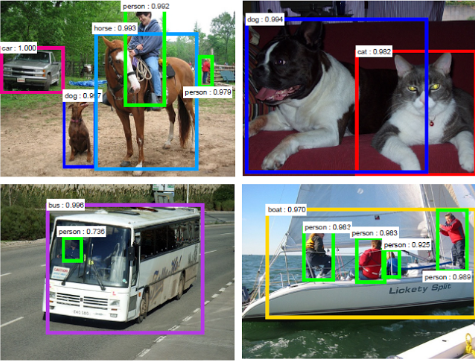
\includegraphics[width=0.5\textwidth]{images/bus.png}
       \begin{itemize}
           \item Proposals are the test-time computational bottleneck in state-of-the-art detection systems
           \item Object detection is driven by the success of region proposal methods (Selective Search and EdgeBoxes) and R-CNN. But it is still relatively slow.
           \item This paper proposes RPN that shares convolutional layers to achieve nearly cost-free computing (10ms/image)
       \end{itemize}
    \end{frame}

    \begin{frame}
     \frametitle{What is a CNN?}
        \centering
          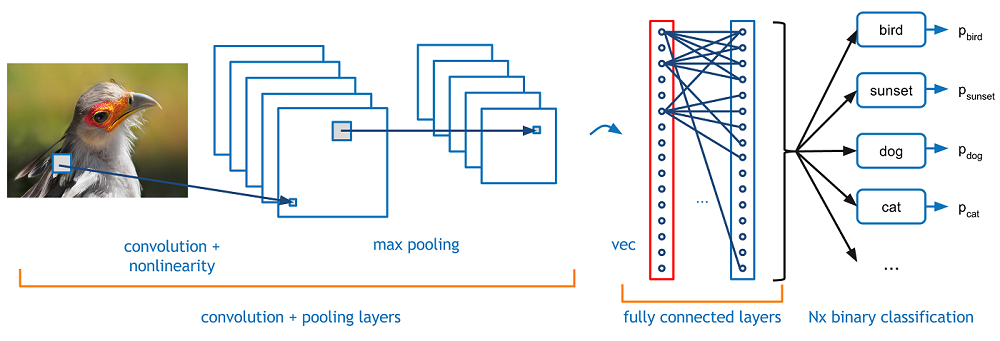
\includegraphics[width=1.0\textwidth]{images/CNN.png}
           \begin{itemize}
           \item When a computer sees an image (takes an image as input), it will see an array of pixel values
           \item  Each of these numbers is given a value from 0 to 255 which describes the pixel intensity at that point
           \item The idea is that you give the computer this array of numbers and it will output numbers that describe the probability of the image being a certain class (.80 for cat, .15 for dog, .05 for bird, etc)
       \end{itemize}
      
    \end{frame}
    
    \begin{frame}
       \frametitle{CNN- Convolutional Layer}
        \centering
          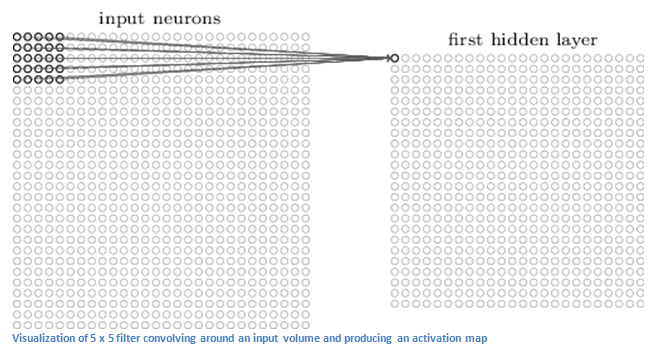
\includegraphics[width=0.5\textwidth]{images/convlayer.png}
        
          \begin{itemize}
           \item  The flashlight is called a filter(or sometimes referred to as a neuron or a kernel) and the region that it is shining over is called the receptive field
           \item As the filter is sliding, or convolving, around the input image, it is multiplying the values in the filter with the original pixel values of the image (aka computing element wise multiplications)
           \item These multiplications are all summed up. So now you have a single number
           \end{itemize}
    \end{frame}
    
    \begin{frame}
       \frametitle{CNN- Pooling Layer}
        \centering
          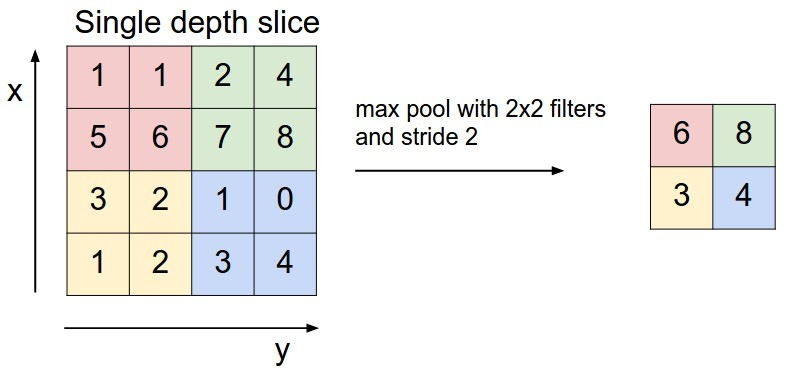
\includegraphics[width=1.0\textwidth]{images/maxpool.jpeg}
    \end{frame}

    \begin{frame}
       \frametitle{CNN- Fully Connected Layer}
        \centering
          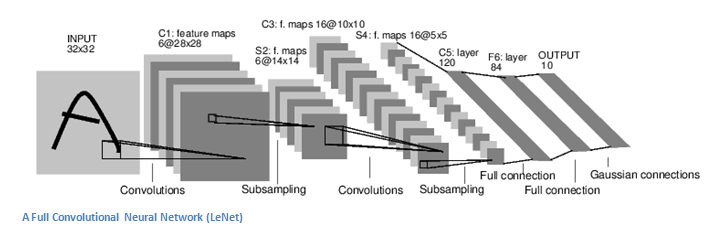
\includegraphics[width=1.0\textwidth]{images/LeNet.png}
          \begin{itemize}
           \item This layer basically takes an input volume (whatever the output is of the conv or ReLU or pool layer preceding it) and outputs an N dimensional vector where N is the number of classes that the program has to choose from
       \end{itemize}
    \end{frame}
    
    \begin{frame}
       \frametitle{Linear Classifier}
        \centering
          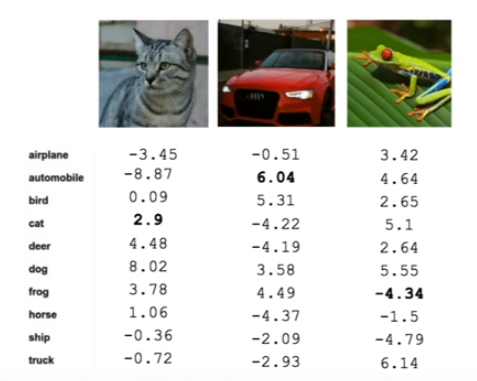
\includegraphics[width=0.5\textwidth]{images/linearclassifier.PNG}
          \begin{itemize}
              \item The way this fully connected layer works is that it looks at the output of the previous layer (which as we remember should represent the activation maps of high level features) and determines which features most correlate to a particular class
          \end{itemize}
    \end{frame}
    
    \begin{frame}
       \frametitle{CNN- Training}
        \centering
          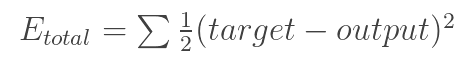
\includegraphics[width=1.0\textwidth]{images/Equation.png}
    \end{frame}
    
    \begin{frame}
       \frametitle{What is a RPN?}
       \centering
        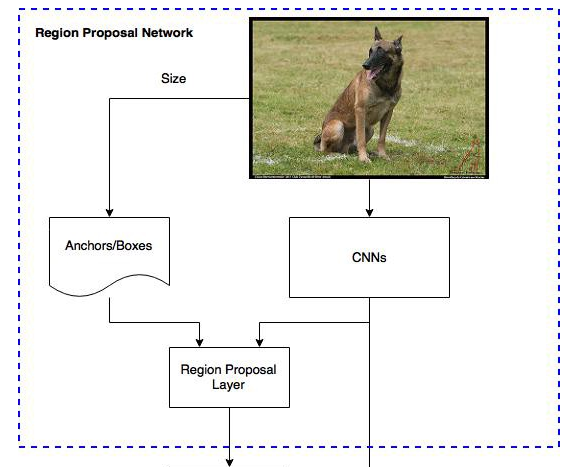
\includegraphics[width=0.5\textwidth]{images/rpn.PNG}
        \begin{itemize}
            \item The output of a region proposal network (RPN) is a bunch of boxes/proposals that will be examined by a classifier and regressor to eventually check the occurrence of objects
        \end{itemize}
    \end{frame}
    
     \begin{frame}
        \frametitle{R-CNN, Fast R-CNN, Faster R-CNN}
        \begin{columns}
            \begin{column}{1.0\textwidth}
              \begin{column}{0.4\textwidth}
                  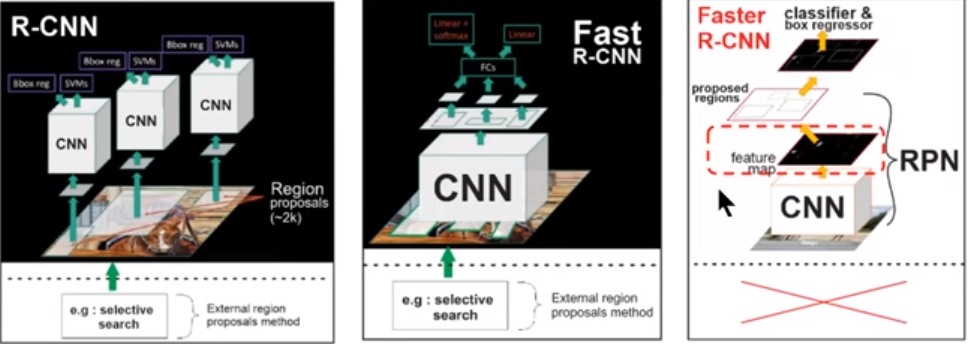
\includegraphics[width=2.5\textwidth]{images/RCNN.png}
                  \begin{center}
                  \end{center}
            \end{column}
            \begin{center}
            \begin{tabular}{c rrr} 
            \hline
              & R-CNN & Fast R-CNN & Faster R-CNN \\ 
            \hline
            Time Per Image & 50s & 2s & 0.2s \\ 
            \hline
            Speed-up & 1x & 25x & 250x\\ 
            \hline
            \end{tabular}
            \end{center}
            \end{column}
        \end{columns}
    \end{frame}
    
    \begin{frame}
       \frametitle{Architecture}
       \centering
         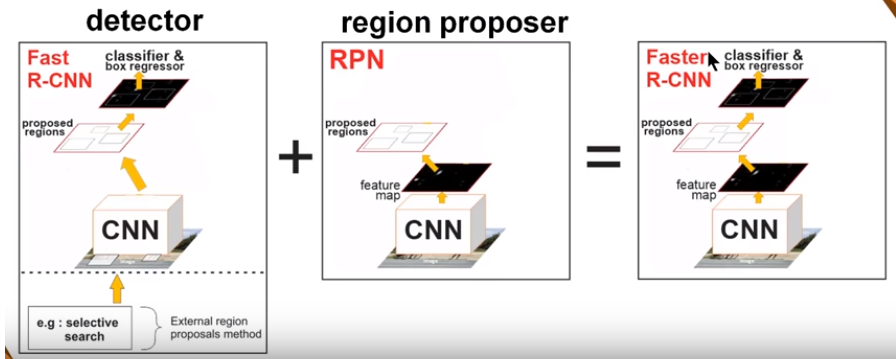
\includegraphics[width=1.0\textwidth]{images/architecture.PNG}
    \end{frame}
    
    \begin{frame}
       \frametitle{ZFnet}
       \centering
         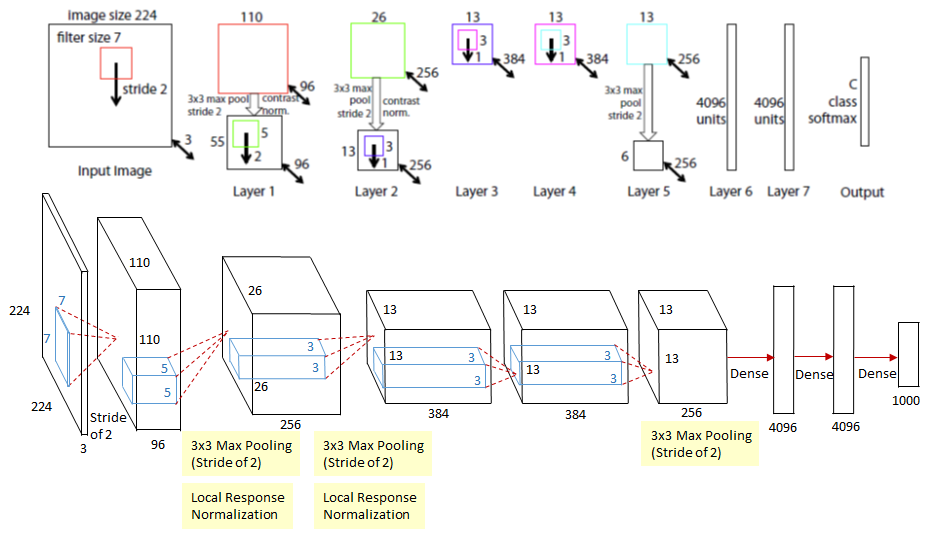
\includegraphics[width=1.0\textwidth]{images/zfnet.png}
    \end{frame}
    
    \begin{frame}
       \frametitle{VGG-16}
       \centering
         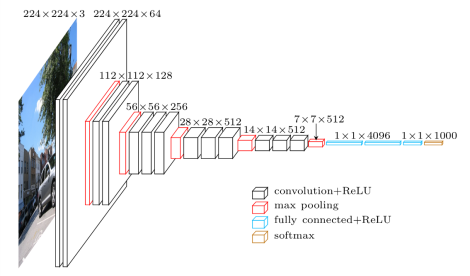
\includegraphics[width=1.0\textwidth]{images/vgg.png}
    \end{frame}
    
    
    \begin{frame}
       \frametitle{Share Parameters}
       \centering
         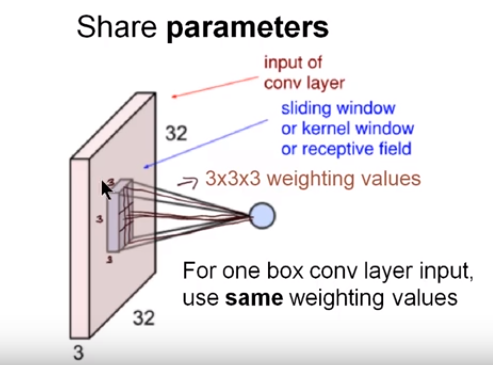
\includegraphics[width=0.5\textwidth]{images/shareparameters.PNG}
         \begin{itemize}
             \item The RPN and Fast R-CNN use the same weights so we say they share parameters
         \end{itemize}
    \end{frame}
    
    
    
    
     \begin{frame}
       \frametitle{RPN as Region Proposal Network}
       \centering
         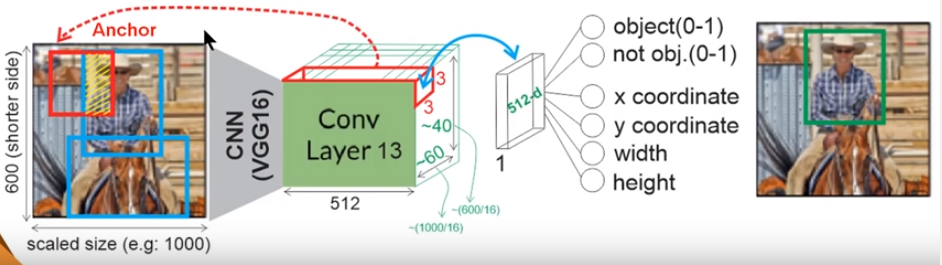
\includegraphics[width=1.0\textwidth]{images/rpnRP.PNG}
    \end{frame}
    
    
    \begin{frame}
       \frametitle{Training}
         \begin{enumerate}
             \item Train RPN: ImageNet pre-trained model
             \item Train detection network with Fast R-CNN: uses proposals generated bu ImageNet pre-trained model
             \item Update Convolutional Layers: fine-tune RPN
             \item Update Convolutional Layers: fine-tune R-CNN
         \end{enumerate}
    \end{frame}
    
    \begin{frame}
       \frametitle{Training}
         \title{Training Properties}
         \begin{enumerate}
             \item Weighting value initialization:N(0, 0.01(squared))
             \item Learning Rate: 0.001 for 60k mini-batch and 0.0001 for next 20k
             \item Learning Update Scheme: momentum update 0.9
             \item Update Convolutional Layers: fine-tune RPN
             \item Update Convolutional Layers: fine-tune R-CNN
         \end{enumerate}
    \end{frame}
    
    \begin{frame}
       \frametitle{Training: Step 1 (RPN)}
       \centering
         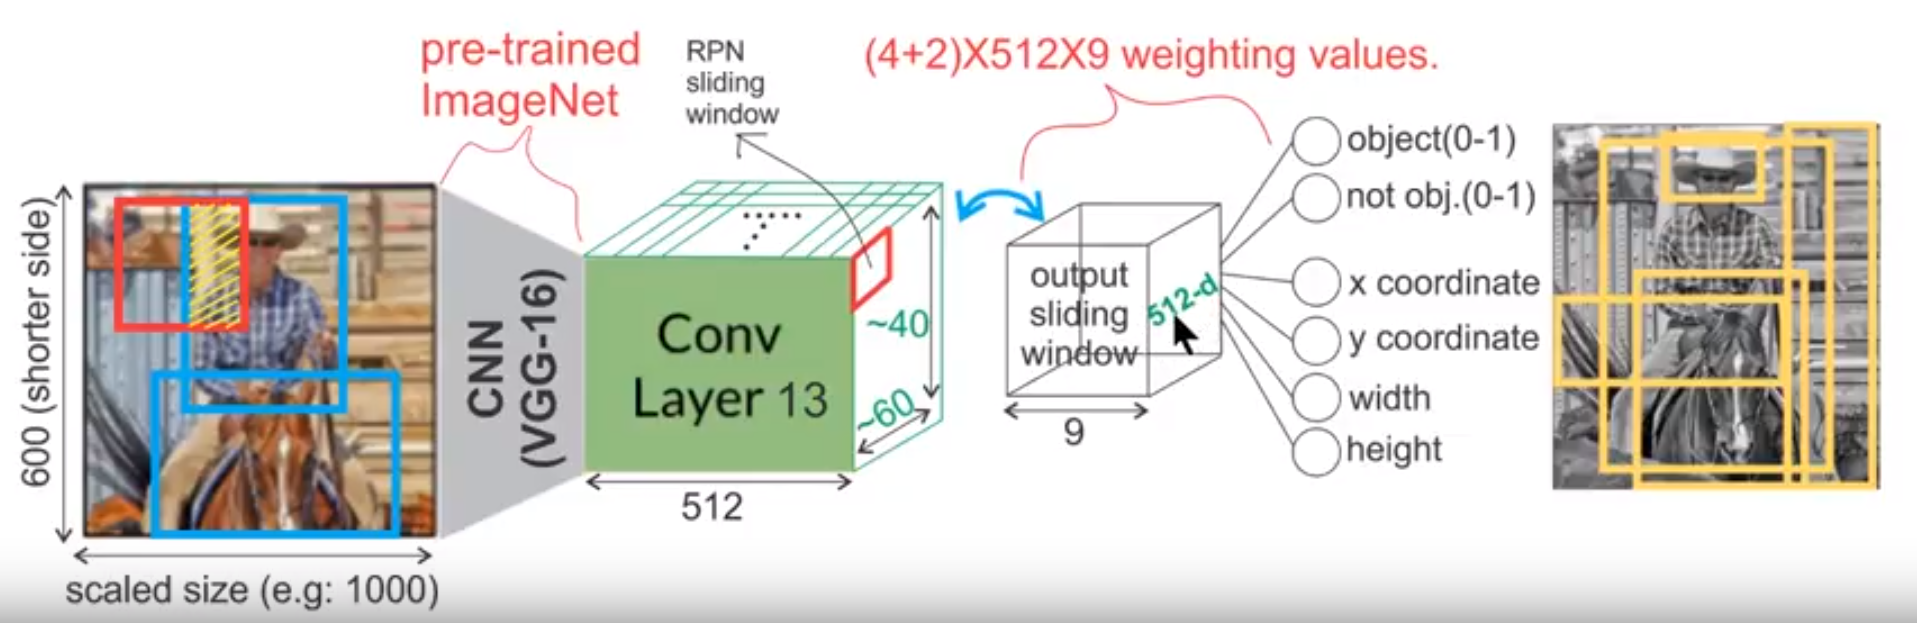
\includegraphics[width=1.0\textwidth]{images/training.PNG}
    \end{frame}
    
    \begin{frame}
       \frametitle{Training: Step 1 cont...}
       \centering
         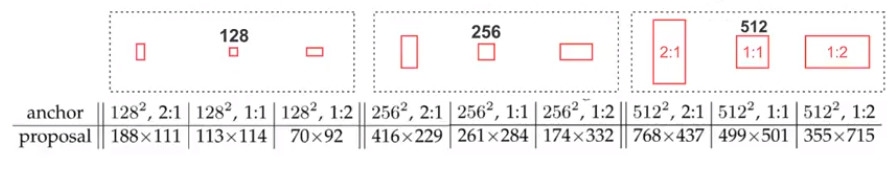
\includegraphics[width=1.0\textwidth]{images/anchors.PNG}
    \end{frame}
    
    \begin{frame}
       \frametitle{Training: Step 2 (detector)}
       \centering
         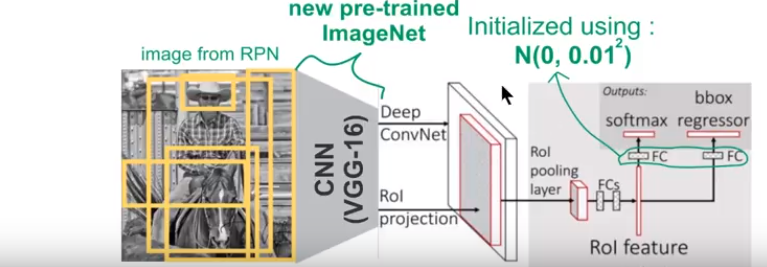
\includegraphics[width=1.0\textwidth]{images/step2.PNG}
    \end{frame}
    
    \begin{frame}
       \frametitle{Training: Step 3 (RPN)}
       \centering
         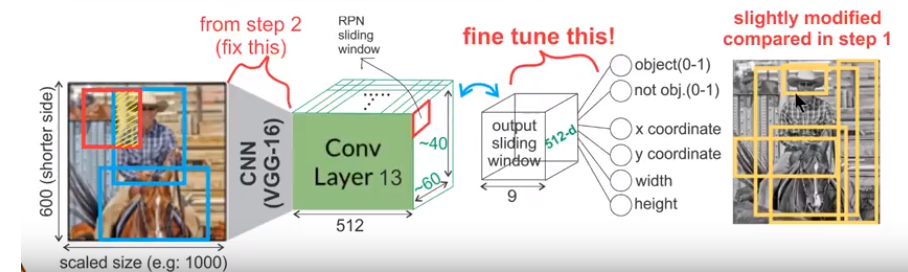
\includegraphics[width=1.0\textwidth]{images/step3.PNG}
    \end{frame}
    
        \begin{frame}
       \frametitle{Training: Step 4 (detector)}
       \centering
         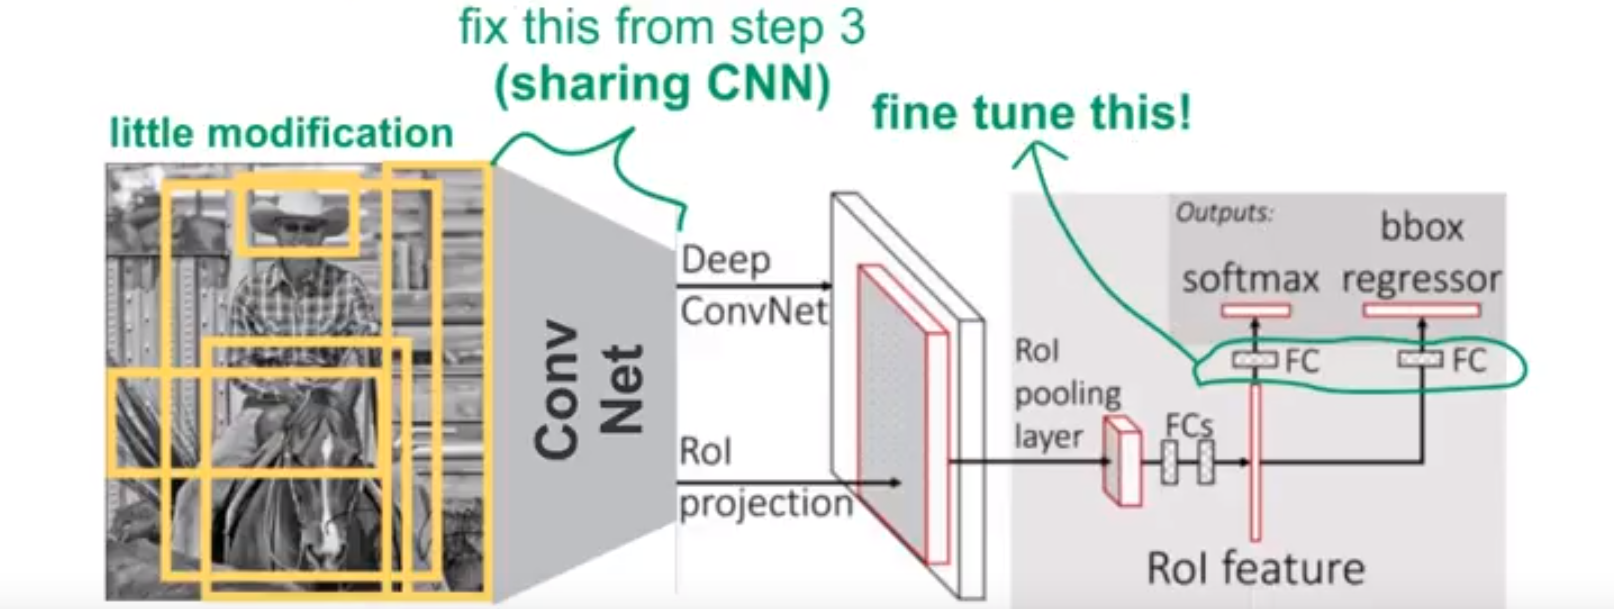
\includegraphics[width=1.0\textwidth]{images/step4.PNG}
    \end{frame}
    
    \begin{frame}
       \frametitle{PASCAL VOC 2007}
       \centering
         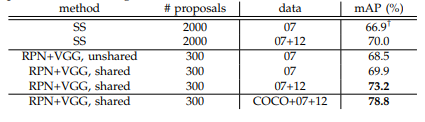
\includegraphics[width=1.0\textwidth]{images/t1.PNG}
    \end{frame}
    
    \begin{frame}
       \frametitle{PASCAL VOC 2012}
       \centering
         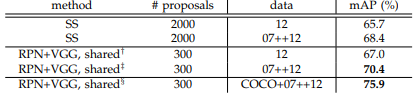
\includegraphics[width=1.0\textwidth]{images/t2.PNG}
    \end{frame}
    
    \begin{frame}
       \frametitle{Timing(ms) on a K40 GPU}
       \centering
         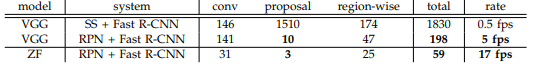
\includegraphics[width=1.0\textwidth]{images/t3.PNG}
    \end{frame}
    
    
    
    
\end{document}